\Chapter{Megvalósítás}
\iffalse
Ez a fejezet mutatja be a megvalósítás lépéseit.
Itt lehet az esetlegesen előforduló technikai nehézségeket említeni.
Be lehet már mutatni a program elkészült részeit.

Meg lehet mutatni az elkészített programkód érdekesebb részeit.
(Az érdekesebb részek bemutatására kellene szorítkozni.
Többségében a szöveges leírásnak kellene benne lennie.
Abból lehet kiindulni, hogy a forráskód a dolgozathoz elérhető, azt nem kell magába a dolgozatba bemásolni, elegendő csak behivatkozni.)

A dolgozatban szereplő forráskódrészletekhez külön vannak programnyelvenként stílusok.
Python esetében például így néz ki egy formázott kódrészlet.
\begin{python}
import sys

if __name__ == '__main__':
    pass
\end{python}

A stílusfájlok a \texttt{styles} jegyzékben találhatók.
A stílusok között szerepel még C++, Java és Rust stílusfájl.
Ezek használatához a \texttt{dolgozat.tex} fájl elején \texttt{usepackage} paranccsal hozzá kell adni a stílust, majd a stílusfájl nevével megegyező környezetet lehet használni.
További példaként C++ forráskód esetében ez így szerepel.
\begin{cpp}
#include <iostream>

class Sample : public Object
{
    // An empty class definition
}
\end{cpp}
Stílusfájlokból elegendő csak annyit meghagyni, amennyire a dolgozatban szükség van.
Más, C szintaktikájú nyelvekhez (mint például a JavaScript és C\#) a Java vagy C++ stílusfájlok átszerkesztésére van szükség.
(Elegendő lehet csak a fájlnevet átírni, és a fájlban a környezet nevét.)

Nyers adatok, parancssori kimenetek megjelenítéséhez a \texttt{verbatim} környezetet lehet használni.
\begin{verbatim}
$ some commands with arguments
1 2 3 4 5
$ _
\end{verbatim}

A kutatás jellegű témáknál ez a fejezet gyakorlatilag kimaradhat.
Helyette inkább a fő vizsgálati módszerek, kutatási irányok kaphatnak külön-külön fejezeteket.
\fi
\section{Szerveroldal megvalósítása}

A szerveroldali alkalmazás a Node.js által szolgált környezetben, az Express.js(5.2.1) keretrendszer segítségével van elkészítve. A Node.js biztosítja a JavaScript kód futását, amíg az Express.js a kliensoldalról érkező HTTP-kérések kezelését és az API végpontok megalkotásában segít. A szerver feladata a beérkező kérések feldolgozása, az ezekhez kapcsolódó műveletek végrehajtása, valamint a műveletek végeredményeinek kiszolgálása a kliensoldal számra. 
Felépítésében a program az több fájlba és mappára tagolódik, amelyek külön feladatkörökre vannak osztva.
\begin{itemize}
\item A működésének központi eleme az app.js fájl amely az Express alkalmazás létrehozásáért felel,
\item a konfigurációs beállítások a helyi futáshoz a .env fájlban találhatóak,
\item az API végpontokhoz tartozó útvonalak és a kérések feldolgozása a routes mappában szereplő fájlokba lettek kiszervezve,
\item a middleware mappában a kérések feldolgozásához szükséges saját definiálású köztes függvények kerülnek,
\item végül a models mappában találhatóak azon modellek, amelyek meghatározzák az adatbázisban tárolt dokumentumok szerkezetét. 
\end{itemize}
A funkciók ilyen formában történő elkülönítésével a program felépítése áttekinthető és jól karbantartható kódot eredményez. A program a megvalósításhoz a bcrypt(6.0.0), cookie-parser(1.4.7), cors(2.8.6), dotenv(17.4.1), jsonwebtoken(9.0.3) (innentől kezdve jwt) és mongoose(9.3.1) függőségek lettek alkalmazva az express.js(5.2.1) mellet.

A szerver indításakor először létrejön az Express alkalmazás, majd megtörténik a konfigurálása. A konfigurálásban a saját portja, a cors, a cookie-parser és a express.json middleware-k kerülnek beállításra, majd ha a környezeti változóban megvan adva, akkor a fordított proxy alkalmazását engedélyezi. A konfigurálás után beállítja az API útvonalait az \texttt{app.use()} parancssal. A felhasználók kezeléséért a /users, a sémák kezeléséért a /projects, míg a beküldött űrlapokhoz kapcsolódó műveletekért a /filledForms útvonal felel. Végül kapcsolódik az adatbázishoz, és ha ez sikeresen megtörténik csak akkor kezd el figyelni a megadott portra.

\subsection{Környezeti változók kezelése}

A szerver konfigurációjához a dotenv(17.4.1) csomag lett alkalmazva. Ez lehetővé teszi, hogy a programhoz egy .env fájl készülhessen, amiből környezeti változókat tölthet be a program. Ezek a fájlban \texttt{VALTOZO=ERTEK} formában vannak leírva, és csak szöveges tartalom tárolására alkalmasak. A benne szereplő változók:
\begin{itemize}
\item a \texttt{ACCESS\_TOKEN\_SECRET} aminek értéke a felhasználó hitelesítésében használt tokenek titkos kulcsa,
\item a \texttt{DATABASE\_URL} aminek értéke az adatbázis kapcsolati karakterlánca, fejlesztői környezetben ez \texttt{mongodb://localhost:27017/XmlFormMaker} jelent,
\item a frontend címe \texttt{FRONTEND\_URL}, aminek fejlesztői környezetben az értéke \texttt{http://localhost:4200}
\item a saját portja \texttt{Port}, amin a bejövő kéréseket figyeli, értéke \texttt{3000},
\item végül a \texttt{TRUST\_PROXY}, ami beállítja, hogy egy fordított proxy-n keresztül jönnek-e a kérések, aminek értéke \texttt{FALSE}
\end{itemize} 
Ezeknek a változóknak a program élesben történő futtatásához, a futtatókörnyezet alapján kell megadni az értékeket. A környezeti változók használatának előnye, hogy a konfigurációs értékeket nem szükséges közvetlenül a forráskódban megadni. A fejlesztési és éles környezet eltérő beállításokkal működhet anélkül, hogy a programkódot módosítani kellene.

\subsection{A köztes szoftverek}
Az Express alkalmazás a különböző kérések feldolgozásához több middleware-t használ. Ezek olyan függvények, amelyek a kérés és a válasz közötti feldolgozási folyamatba kapcsolódnak be.

A CORS(2.8.6) (Cross-Origin Resource Sharing) egy olyan middleware, amivel engedélyt lehet adni a böngésző számára, hogy egy webalkalmazásban az express mely más eredetű szerverekről kaphat kéréseket. Mivel a program szétválasztott architektúraként van megalkotva, vagyis a kliensoldal és a szerveroldal külön szerveren fut, a kettő eltérő eredetűnek számít. CORS beállítása nélkül a böngésző Same-Origin Policy szabályai megakadályoznák, hogy a kliensoldal szabadon hozzáférjen a szerver válaszaihoz.
\begin{java}
app.use(cors({
    origin: process.env.FRONTEND\_URL,
    credentials: true
}));
\end{java}
A konfigurációban az origin beállítás határozza meg, hogy melyik kliensoldali címről érkező kérések engedélyezettek. Ennek értéke a FRONTEND\_URL környezeti változóban van megadva. A credentials: true beállítás pedig lehetővé teszi a hitelesítési sütik továbbítását a kérésekkel együtt, ami szükséges az alkalmazás JWT alapú, HTTP-only sütiben tárolt hitelesítéséhez.
Ennek használatát kilehetne váltani az Angular alkalmazás és az API azonos eredet alatt történő kiszolgálásával vagy egy olyan middleware írásával ami beállítja a HTTP fejléceinek adatait, de ezek szükségtelen bonyolítások lennének.

A cookie-parser(1.4.7) csomag a HTTP kérések fejlécében érkező sütik feldolgozására szolgál. Ennek segítségével a szerver egyszerűen hozzáférhet a kliensoldal által küldött sütik értékeihez. Az alkalmazásban erre a JWT token kiolvasása miatt van szükség, mivel a felhasználó hitelesítésére szolgáló token HTTP-only sütiben kerül tárolásra.

Az \texttt{express.json()} middleware az Express beépített funkciója, amely lehetővé teszi a JSON formátumban érkező kéréstörzsek automatikus feldolgozását. Ennek köszönhetően a szerver az elküldött adatokat a req.body objektumon keresztül elérheti. Ezelőtt erre a célra a külön body-parser csomag volt gyakran használatban, azonban az Express most már saját megoldást biztosít erre a feladatra, így nincs erre szükség.

\subsection{Az adatbázis-kapcsolat és a szerver indítása}

A szerver működéséhez szükséges a MongoDB adatbázishoz való kapcsolódás is. Ezt a mongoose(9.3.1) csomag biztosítja, amely magasabb szintű interfészt kínál a MongoDB kezeléséhez, könnyíti az adatok létrehozását, lekérdezését, módosítását és törlését. A Mongoose egyik legfontosabb funkciója a sémák és modellek létrehozása. A séma meghatározza az adott dokumentumtípus felépítését, például a mezők nevét, adattípusát, és a megszorításokat. Ilyen megszorítás lehet egy mező kötelezővé tétele, minimális vagy maximális hosszának meghatározása, vagy egyedi érték előírása. A sémák alapján modellek hozhatóak létre, amelyek az adott dokumentumtípus adatbázisbeli kezeléséért felelnek. A modellek segítségével végezhetőek el különböző adatbázis műveletek.

A Mongoose emellett támogatja egyedi metódusok definiálását is. A sémákhoz statikus metódusok rendelhetők, amelyek közvetlenül a modellből hívhatók meg, amíg az egyedi példánymetódusok az adott dokumentumhoz kapcsolódik. Ez lehetőséget biztosít arra, hogy az adatkezeléshez kapcsolódó műveletek ne kizárólag az útvonalakban jelenjenek meg, hanem az adott modellhez kapcsolódóan legyenek definiálva. 

Az alkalmazásban a Mongoose segítségével három fő modell került kialakításra, amik segítségével épül fel az adatbázis: a felhasználók, a projektek és a beküldött űrlapok kezelésére szolgáló modellek. Ezek részletes felépítése, mezői és a közöttük fennálló kapcsolatok az adatbázis bemutatásánál lesznek ismertetve.

A kapcsolat létrehozásához a mongoose.connect() metódus szolgál, amelynek a DATABASE\_URL környezeti változóban megadott kapcsolati karakterláncot kell átadni. A kapcsolat sikeres létrejötte után a mongoose-t beállítja, hogy csak a sémákban szereplő mezőket engedje lekérdezne, és csak ez után kezdi meg a beérkező HTTP kérések fogadását. A szerver által használt portszámot a PORT környezeti változó határozza meg, amelynek hiányában az alkalmazás alapértelmezés szerint a 3000-es portot használja.

\begin{java}
async function main() {
    await mongoose.connect(process.env.DATABASE_URL);
    mongoose.set("strictQuery", true);

    app.listen(PORT, (error) => {
    	if(!error){
        	console.log("Server listening at:",PORT)
    	}else{
        	console.log("An error occured",error);
    	}
	})
}
\end{java}

\section{Adatbázis felépítése}

A MongoDB adatbázis három gyűjteményre van felosztva, a \texttt{users} gyűjtemény, amiben a felhasználók adatai vannak, a \texttt{projects} amiben a felhasználók által feltöltött XML-sémák kerülnek tárolásra, valamint a \texttt{filledforms} gyűjtemény ahol a beküldött űrlapok vannak lementve. Ezek kezelését a backendben a Mongoose könyvtár segítségével megvalósított modellek végzik. Ez lehetőséget ad az egyes mezők típusainak meghatározásához legyenek tárolva, valamint az azokhoz tartozó megszorítások, például a kötelező mezők, egyedi értékek, vagy egyéb szabályok.

A \texttt{UserSchema} modell dokumentuma hat mezőből áll. Az elsődleges kulcs a \texttt{\_id}, amit az adatbázis automatikusan generál, ennek típusa a MongoDB BSON adatformátumának ObjectId típusa, amely egy 12 bájtos egyedi azonosító. Szöveges formában 24 karakterrel ábrázolható. A Mongoose által kezelt dokumentumok ezenkívül alapértelmezés szerint egy egész szám típusú, \texttt{\_\_v} nevű verziómezőt is tartalmaznak, amely a dokumentum verziójának nyilvántartására szolgál. Bár minden minden gyűjteményben megtalálható, a program nem veszi használatba a mezőt. A \texttt{name} mezőben található a felhasználó név karakterláncként mentve, ezeknek minimum négy karakter hosszúnak és egyedieknek kell lenni, ezen felül kisbetűkre van cserélve minden karaktere tárolás előtt. A \texttt{password} mezőben a már hash-elt jelszavak hasonlóképpen karakterláncban vannak tárolva és legalább nyolc karakter hosszúnak kell lenniük. A gyűjtemény ezeken kívül dátum adattípusban számon tartja a dokumentum létrehozásának dátumát a \texttt{createdAt} mezőben és az utolsó bejelentkezés időpontját a \texttt{lastLogin} mezőben. Mindkét dátum típusú mező a jelenlegi időpontot tárolja alapértelmezés szerint egy új dokumentum létrehozásakor, ha nincs külön megadva.

A \texttt{projectSchema} modell dokumentuma az adatbázisban hét mezőként jelenik meg. Az automatikusan létrehozott \texttt{\_id} és \texttt{\_\_v} mellet benne van a \texttt{name} mező amiben a séma neve van karakterláncként tárolva, míg a \texttt{schema} magát a sémát tárolja, szintén karakterlánc formájában, ezeknek a megadása kötelező. A \texttt{formCreator} egy kötelező mező, ami sémát létrehozó felhasználó azonosítóját tartalmazza, ez az idegen kulcs szerepét szolgálja lekérdezésekben. A dokumentum létrehozásának időpontját a \texttt{createdAt}, amíg az utolsó módosítás időpontját az \texttt{updatedAt} mező tartja számon. Mindkét mező dátum típusú, és értékük alapértelmezés szerint a dokumentum létrehozásakor a jelenlegi időpontra áll be.

A \texttt{filledFormsSchema} modell dokumentuma hasonlóan hét mezőből áll, amiből kettő az a \texttt{\_id} és \texttt{\_\_v} mezők. A \texttt{form} mezőben a beküldött XML dokumentumot tárolja karakterlánc formájában. A \texttt{schema} és a \texttt{formCreator} mezők a séma és a sémaalkotójának azonosítóját tartalmazza karakterlánc formájában, amik idegenkulcsokként szolgálnak. A \texttt{formSubmitter} a kitöltést elvégző felhasználó nevét tárolja karakterlánc formájában, amennyiben be van jelentkezve. Végül a \texttt{createdAt} mező dátum típusban tartja nyilván a beküldés időpontját, amely alapértelmezésben a dokumentum létrehozásának időpontja.

A gyűjtemények közti kapcsolatot az egyes dokumentumokban tárolt azonosítók biztosítják.
\begin{itemize}
\item A \texttt{users} és a \texttt{projects} között egy-több kapcsolat van, hiszen több sémát is feltölthet a felhasználó,
\item a \texttt{users} és \texttt{filledforms} között megint egy-több kapcsolat van, mert több válasz XML-t kaphat a felhasználó,
\item végül a \texttt{projects} és a \texttt{filledforms} között is egy több, mivel egy űrlaphoz több választ is beküldhetnek.
\end{itemize}
Ezeket a kapcsolatokat az adott gyűjtemények mezőit a \ref{fig:relaciosDiagram}. ábra relációs sémája szemlélteti.

\begin{figure}[h]
\centering
\frame{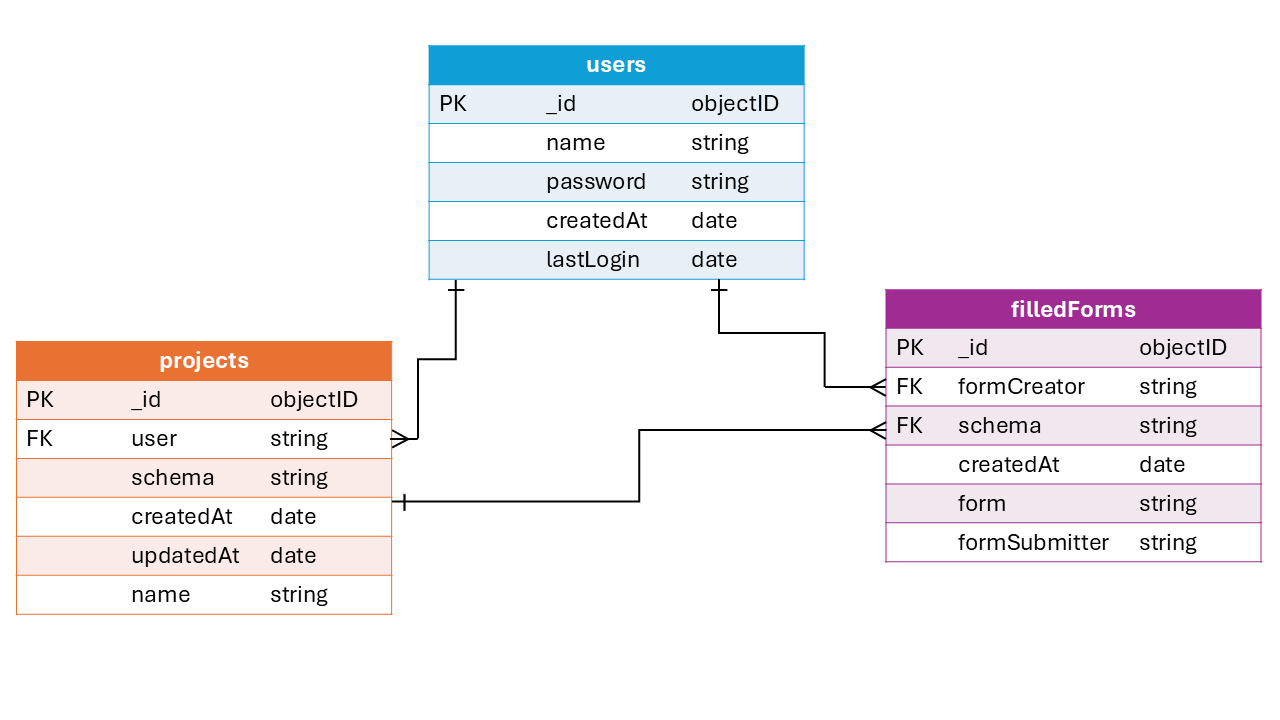
\includegraphics[width=\textwidth]{images/relaciosDiagram.png}}
\caption{Az adatbázis relációs sémája.}
\label{fig:relaciosDiagram}
\end{figure}

\section{Felhasználók kezelése és hitelesítés a szerveren}

A felhasználók kezeléséért felelős kérések a \texttt{/users} útvonalhoz kapcsolódva végződnek. Ezek külön útvonalmodulban találhatók, amely az Express-nek a Router funkciója használja. A felhasználói adatok kezeléséhez a korábban bemutatott User Mongoose modell kerül felhasználásra.

A hitelesítés megvalósításához a rendszer a JWT(9.0.3) technológiát használ, ami lehetővé teszi, hogy a felhasználókat a program azonosítja anélkül, hogy a minden kérésnél megadják a felhasználói adataikat. A JWT egy nyílt szabványon alapuló tokenformátum, amely lehetővé teszi az adatok biztonságos továbbítását két fél között.  A JWT előnye, hogy a szervernek nem szükséges külön adatokat tárolnia a felhasználó bejelentkezési állapotának fenntartásához, mivel az azonosításhoz szükséges információkat maga a token tartalmazza. A token érvényessége annak aláírása és lejárati ideje alapján ellenőrizhető.
\begin{java}
const maximumAge = 3 * 24 * 60 * 60;
const createToken = (id) => {
    return jwt.sign({ id }, process.env.ACCESS_TOKEN_SECRET, {
        expiresIn: maximumAge
    });
};
\end{java}
A token a felhasználó egyedi azonosítóját tárolja, hitelességét pedig a szerver egy titkos kulcs segítségével írja alá és ellenőrzi. A token három nap után jár le, másodpercben megadva.
A jelszavak biztonságáért a bcrypt(6.0.0) könyvtár felelős, ami a jelszavakat egyirányúan hash-eli az adatbázisba mentés előtt. A keletkezett 60 karakterből álló szöveges karakterlánc tartalmazza az algoritmus verziószámát és a számítási költségtényezőt, egy véletlenszerűen generált sót, és magát a titkosított jelszót.

\subsection{Regisztráció}

A regisztráció a \texttt{/users/signup} útvonalra küldött POST kéréssel történik. A szerver a kérés törzsében (req.body) megkapja meg a felhasználó által regisztrációkor megadott adatokat, amelyek alapján létrehoz egy új User példányt.

A jelszó mentés előtt ellenőrzi, hogy legalább nyolc karakter hosszúságú legyen. Ez után a bcrypt segítségével létrehozz egy véletlenszerű sót, amit a könyvtár a jelszó hash-elése során használ. A hash-elt jelszó kerül az adatbázisba,ezért az eredeti jelszó nem tárolódik közvetlenül.

A felhasználó sikeres mentése után a szerver létrehoz egy JWT-t, amely a felhasználó adatbázisbeli dokumentumának azonosítóját tartalmazza. A token a jwt nevű egy sütiben kerül elküldésre a kliens számára.
\begin{java}
const cookieOptions = {
    httpOnly: true,
    maxAge: maximumAge * 1000,
    secure: true,
    sameSite: "lax",
    path: "/",
};
await res.cookie("jwt", token, cookieOptions);
\end{java}
A \texttt{httpOnly} beállítás megakadályozza, hogy a kliensoldali JavaScript kód közvetlenül hozzáférjen a süti tartalmához. A \texttt{maxAge} süti érvényességi idejét adja meg ezredmásodpercben, ami három nap, a \texttt{secure} beállítás miatt pedig csak biztonságos HTTPS kapcsolaton keresztül továbbítható. A \texttt{sameSite: "lax"} védelmet nyújt a CSRF (Cross-Site Request Forgery) támadások ellen. A süti csak az ugyanarról a webhelyről induló kéréseknél, illetve biztonságos külső navigációnál kerül elküldésre. A \texttt{path: "/"} pedig beállítja, hogy a süti a weboldal teljes domainjén, minden útvonalon és aloldalon elérhető lesz.

Akkor, ha a regisztráció sikeres, akkor a szerver egy 201 státuszkódot küld vissza a kliensoldalra, viszont ha a megadott felhasználónév foglalt, az adatbázis egyedi mezőkre vonatkozó megszorítása miatt a művelet sikertelen vagy egyéb hiba történik, akkor egy hibaüzenetet küld vissza.

\subsection{Bejelentkezés}

A bejelentkezés a \texttt{/users/login} útvonalra küldött POST kéréssel történik. A szerver megkapja a felhasználónevet és jelszót, majd meghívja rá a \texttt{User} modell login statikus metódusát. 

A metódus elsőnek megkeresi a felhasználó név alapján a megfelelő dokumentumot \texttt{this.findOne({name:name.toLowerCase()})}, majd összehasonlítja a talált dokumentum jelszavát a megadott jelszóval a bcrypt segítségével \texttt{const auth = await bcrypt.compare(password,user.password)}. Abban az esetben ha igaz értéket ad vissza akkor a metódus vissza adja az egész dokumentumot, ha nem találja a felhasználót vagy a jelszó helytelen akkor hibát dob.

A sikeres ellenőrzés után, a megkapott dokumentum alapján a regisztrációhoz hasonlóan  létrehozza a felhasználóhoz tartozó JWT-t, amit egy sütiben küld vissza. A bejelentkezés időpontja az adatbázisban rögzítésre kerül, majd a szerver visszajelzést küld a kliensnek.

\subsection{Kijelentkezés}

A kijelentkezés a \texttt{/users/logout} útvonalra küldött POST kéréssel történik. Mivel a hitelesítési token a böngésző sütijében található, a szerver a \texttt{res.clearCookie("jwt", {httpOnly: true, secure: true, sameSite: "lax", path: "/",})} metódus segítségével törli azt. A törlés során ugyanazokat a fontos süti-beállításokat alkalmazza, amelyeket a létrehozáskor is használt.

A művelet sikeressége esetén a szerver visszajelzést küld a kliensnek.

\subsection{Bejelentkezési állapot ellenőrzése}

A \texttt{/users/user} útvonal GET kéréssel hívható meg, és annak ellenőrzésére szolgál, hogy a felhasználó rendelkezik érvényes hitelesítési tokennel. A szerver a cookie-parser segítségével hozzáfér a kérésben érkező jwt sütihez, majd a JWT könyvtár \texttt{verify()} metódusával ellenőrzi annak érvényességét.

Az ellenőrzés során a szerver a token aláírását és érvényességi idejét is vizsgálja. Akkor, ha a token érvényes, a válasz jelzi, hogy a felhasználó be van jelentkezve. Hiányzó, lejárt vagy érvénytelen token esetén a szerver a bejelentkezés hiányát jelzi.

\subsection{Felhasználó hitelesítés ellenőrzése}

Bár nem ebben a fájlban van definiálva, egy köztes szoftver tartozik még a hitelesítés témájához. A checkUser metódus feladata, hogy ellenőrizze a beérkező HTTP kérésekhez tartozó JWT érvényességét, és ezzel biztosítsa, hogy bizonyos API végpontokat csak bejelentkezett felhasználók érhessenek el, illetve megadja a végpontnak a felhasználó azonosítóját. Hasonlóképen a bejelentkezési állapot ellenőrzéséhez szerver megkapja a jwt sütit majd a titkosítókulcs segítségével ellenőrzi annak érvényességét, ha ez sikeresen végbemegy, akkor a sütiből kiolvasott azonosítót elmenti \texttt{req.userID = decodedToken.id} majd a \texttt{next()} meghívásával továbbengedi a kérést a következő middleware-nek vagy az útvonalhoz tartozó vezérlőfüggvénynek.

A middleware így lehetővé teszi, hogy a hitelesítés ellenőrzését ne kelljen minden egyes védett API végpontban külön megvalósítani. Ehelyett az adott útvonalakhoz hozzárendelhető a checkUser függvény, ami még az útvonal feldolgozása előtt ellenőrzi a felhasználó bejelentkezési állapotát.

\section{Sémák és dokumentumok kezelése a szerveren}

A további két fontos útvonal a \texttt{/projects} és a \texttt{filledForms} útvonalak. Az előbbi a felhasználók által létrehozott sémák adatait szolgálja, amíg az utóbbi a kitöltött űrlapokból összeállított XML-dokumentumokat kezeli.

Mindkét modul a korábban bemutatott Mongoose modelleket használja az adatbázis műveletek végrehajtásához. Emellett több végpontban is a korábban ismertetett checkUser middleware is alkalmazásra kerül, amely biztosítja, hogy az adott műveleteket csak érvényes hitelesítési tokennel rendelkező felhasználók vehessék igénybe. 

\subsection{Sémák kezelése}

\subsubsection{Sémák lekérdezése}

A felhasználóhoz tartozó sémák lekérdezése a \texttt{/projects/user} útvonalra küldött  GET kéréssel történik. A végpont a checkUser middleware-t használja, ezért a szerver először ellenőrzi a felhasználó hitelesítését. Ez után a \texttt{Project.find()} metódus segítségével lekérdezi azokat a dokumentumokat, amelyek user mezője megegyezik a bejelentkezett felhasználó azonosítójával. Ha a felhasználó nem rendelkezik sémával, akkor a szerver üres tömböt küld vissza.

\subsubsection{Adott séma lekérdezése}

Az adott séma azonosító alapján is lekérdezhető a \texttt{/projects/:id} végponton keresztül. Ez megint egy GET kéréssel érhető el, a szerver a kérés paraméteréből kiolvassa az azonosítót, majd a \texttt{Project.findOne()} metódussal megkeresi a hozzá tartozó dokumentumot. Ez a végpont nem szükséges bejelentkezést, mert az űrlapkitöltő oldalnak is szüksége van a séma adatainak lekérdezésére, ami nyilvánosan elérhető.

\section{Kliensoldal megvalósítása}